%%%%%%%%%%%%%%%%%%%%%%%%%%%%%%%%%%%%%%%%%
% Journal Article
% LaTeX Template
% Version 1.4 (15/5/16)
%
% This template has been downloaded from:
% http://www.LaTeXTemplates.com
%
% Original author:
% Frits Wenneker (http://www.howtotex.com) with extensive modifications by
% Vel (vel@LaTeXTemplates.com)
%
% License:
% CC BY-NC-SA 3.0 (http://creativecommons.org/licenses/by-nc-sa/3.0/)
%
%%%%%%%%%%%%%%%%%%%%%%%%%%%%%%%%%%%%%%%%%

%----------------------------------------------------------------------------------------
%	PACKAGES AND OTHER DOCUMENT CONFIGURATIONS
%----------------------------------------------------------------------------------------

\documentclass[twoside,twocolumn]{article}



\usepackage{blindtext} % Package to generate dummy text throughout this template 

\usepackage[sc]{mathpazo} % Use the Palatino font
\usepackage[T1]{fontenc} % Use 8-bit encoding that has 256 glyphs
\linespread{1.05} % Line spacing - Palatino needs more space between lines
\usepackage{microtype} % Slightly tweak font spacing for aesthetics

\usepackage[english]{babel} % Language hyphenation and typographical rules

\usepackage[hmarginratio=1:1,top=32mm,columnsep=20pt]{geometry} % Document margins
\usepackage[hang, small,labelfont=bf,up,textfont=it,up,figurename=Obrázek,tablename=Tabulka]{caption} % Custom captions under/above floats in tables or figures
\usepackage{booktabs} % Horizontal rules in tables

\usepackage{lettrine} % The lettrine is the first enlarged letter at the beginning of the text

\usepackage{enumitem} % Customized lists
\setlist[itemize]{noitemsep} % Make itemize lists more compact

\usepackage{abstract} % Allows abstract customization
\renewcommand{\abstractnamefont}{\normalfont\bfseries} % Set the "Abstract" text to bold
\renewcommand{\abstracttextfont}{\normalfont\small\itshape} % Set the abstract itself to small italic text

\usepackage{titlesec} % Allows customization of titles
\renewcommand\thesection{\Roman{section}} % Roman numerals for the sections
\renewcommand\thesubsection{\roman{subsection}} % roman numerals for subsections
\titleformat{\section}[block]{\large\scshape\centering}{\thesection.}{1em}{} % Change the look of the section titles
\titleformat{\subsection}[block]{\large}{\thesubsection.}{1em}{} % Change the look of the section titles

%\usepackage{fancyhdr} % Headers and footers
%\pagestyle{fancy} % All pages have headers and footers
%\fancyhead{} % Blank out the default header
%\fancyfoot{} % Blank out the default footer
%\fancyhead[C]{} % Custom header text
%\fancyfoot[RO,LE]{\thepage} % Custom footer text

\usepackage{titling} % Customizing the title section

\usepackage{hyperref}
\usepackage{graphicx} % For hyperlinks in the PDF


%----------------------------------------------------------------------------------------
%	TITLE SECTION
%----------------------------------------------------------------------------------------

\setlength{\droptitle}{-4\baselineskip} % Move the title up

\pretitle{\begin{center}\Huge\bfseries} % Article title formatting
\posttitle{\end{center}} % Article title closing formatting
\title{Heuristika simulovaného ochlazování pro řešení MaxWeightedSAT} % Article title
\author{%
    \textsc{Luboš Zápotočný}\\[1ex] % Your name
    \normalsize České vysoké učení technické v Praze - fakulta informačních technologií \\ % Your institution
    \normalsize \href{mailto:zapotlub@fit.cvut.cz}{zapotlub@fit.cvut.cz} % Your email address
%\and % Uncomment if 2 authors are required, duplicate these 4 lines if more
%\textsc{Jane Smith}\thanks{Corresponding author} \\[1ex] % Second author's name
%\normalsize University of Utah \\ % Second author's institution
%\normalsize \href{mailto:jane@smith.com}{jane@smith.com} % Second author's email address
}
\date{} % Leave empty to omit a date \today
%\renewcommand{\maketitlehookd}{%
%\begin{abstract}
%\noindent \blindtext % Dummy abstract text - replace \blindtext with your abstract text
%\end{abstract}
%}

%----------------------------------------------------------------------------------------

\begin{document}

% Print the title
    \maketitle

%----------------------------------------------------------------------------------------
%	ARTICLE CONTENTS
%----------------------------------------------------------------------------------------


    \section{Úvod}

    Problém splnitelnosti booleovské formule (ozačováno z angličtiny SATISFIABILITY, zkráceně SAT) označuje problém
    nalezení splňujícího (vyhovujícího) ohodnocení logické formule v~konjunktivní normálním formě tak, aby byly všechny její
    klauzule splněné.

    SAT byl první problém o kterém se dokázalo, že je NP-úplný~\cite{CookLevin1971}.
    Tedy pro tento problém neexistuje (za předpokladu P $\neq$ NP) efektivní algoritmus, který by tento problém řešil v polynomiálním čase.
    Jelikož se jedná o NP-těžký (NP-úplné problémy jsou podmnožinou NP-těžkých) problém, lze na tento problém převést instance všech problému ze tříd P a NP.

    MaxWeightedSAT označuje optimalizační verzi hledání SAT ohodnocení zároveň s kritériem pro maximalizace součtu
    vah proměnných ohodnocených 1 (True).
    Problém je tedy rozšířen o atributy $w(x_i)$ pro všechny proměnné $w_i$ reprezentující váhové ohodnocení jednotlivých
    proměnných.

    Tato práce se zaměřuje na řešení výše zmíněného NP-těžkého optimzačního problému pomocí heuristiky simulovaného ochlazování.

    Algoritmus náhodně prochází stavovým prostorem ohodnocení proměnných formule tak, aby maximalizoval součet vah pozitivně
    ohodnocených proměnných a zároveň aby toto ohodnocení splňovanou zadanou formuli.

    Stavový prostor je tedy vektor (pole) boolevských ohodnocení (True/False) jednotlivých proměnných.
    Operátorem přechodu do nového stavu je logická změna jednoho náhodného bitu v tomto vektoru.

    Algoritmus přechází do zlepšíjících stavů a s určitou pravděpodobností přechází také do zhrošujících stavů.
    Tímto postupem se heuristika snaží zamezit uvízní v lokálních extrémech.

    Heuristika začíná s vysokou teplotou, která ovlivňuje mimo jiné také pravděpodobnost přijetí nezlepšujících stavů.
    To vede k velkému prozkoumání stavového prostoru v prvních krocích algoirtmu.
    Každý krok algorimu sníží tuto teplotu o násobek chladícího faktoru (lineárně).
    Tímto chlazením se také snižuje pravděpodobnost přijetí zhrošujícího stavu a heuristika tímto konverguje k nalezení
    optimálního řešení.

%------------------------------------------------


    \section{Implementace}

    Heuristika a experimentální vyhodnocení byly naprogramovány v jazyce Python.
    Při hledání ideálních parametrů heuristiky či efektivity algoritmu není uvažována efektivita jazyka jako takového.
    Všechny metriky jsou univerzálně přenositelné mezi různými hardwarovými platformami.

    Hlavní část heuristiky je zobrazena na obrázku~\ref{fig:main-loop} kde lze nahlédnou, jak algoritmus pracuje.

    \begin{figure}
        \centering
        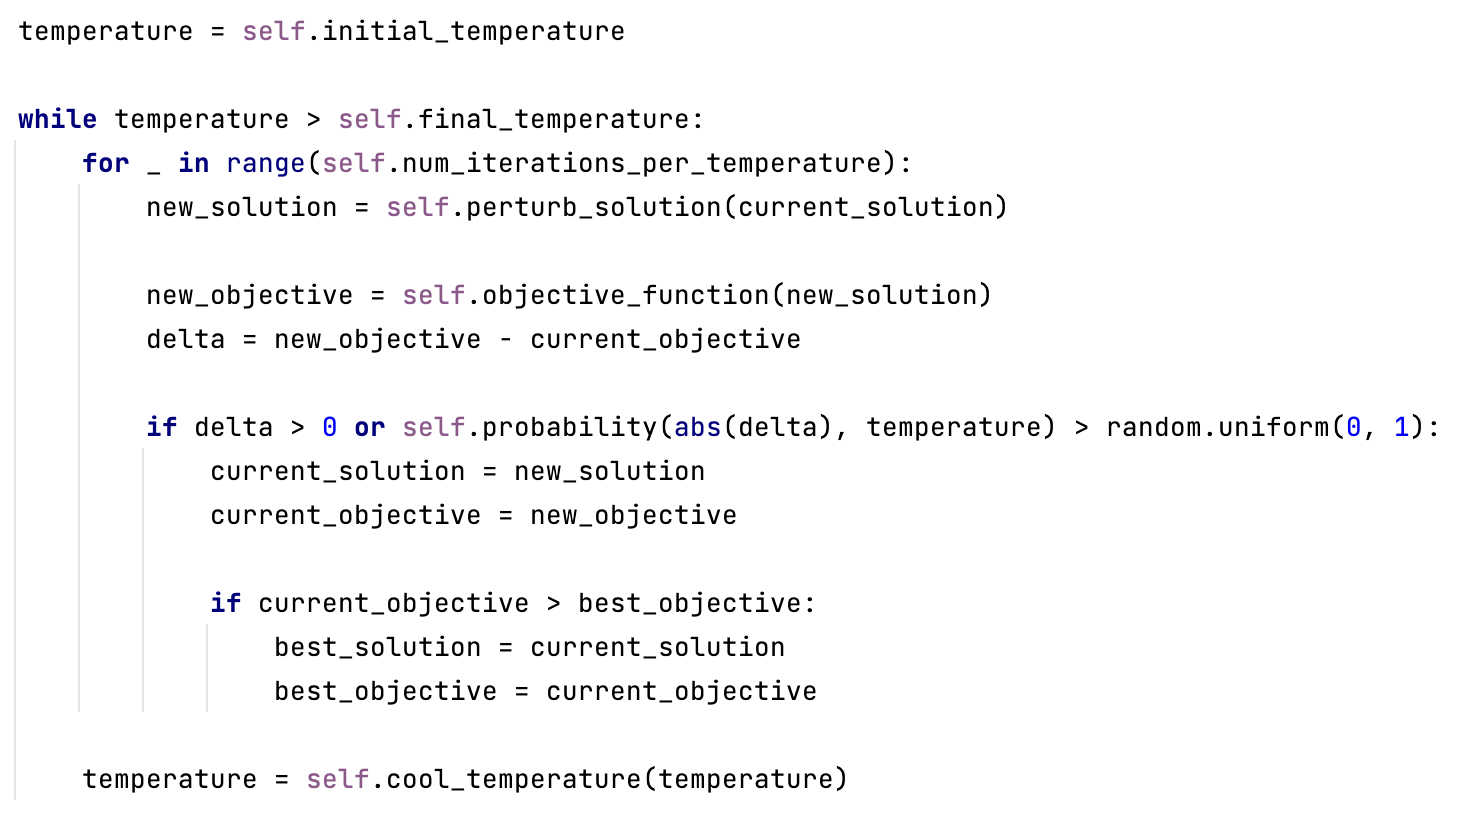
\includegraphics[width=7cm]{images/main-loop}
        \caption{Hlavní smyčka algoritmu}
        \label{fig:main-loop}
    \end{figure}

    Pravděpodobnost přijetí zhoršujícího řešení je závislá na rozdílu hodnot účelové funkce mezi aktuálním řešením a potenciálním novým řešením.
    Zároveň je závislá na aktuální teplotě. Čím větší teplota, tím větší pravděpodobnost, že bude přijato zhoršující řešení.
    Konkrétní implementaci lze vidět na obrázku~\ref{fig:probabilty}.
    Výsledek této funkce je následně v hlavním cyklu porovnán s náhodnou hodnotou v internalu od 0 do 1 a pokud tato hodnota
    převyšuje vygenerovanou náhodnou hodnotu přijímáme zhrošující řešení.

    Zlepšující řešení přijímáme vždy.

    \begin{figure}
        \centering
        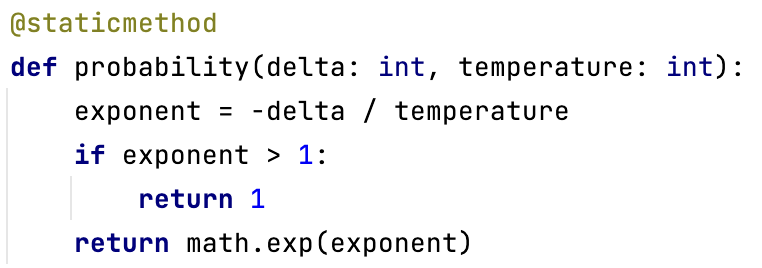
\includegraphics[width=7cm]{images/probabilty}
        \caption{Výpočet pravděpodobnosti přijetí zhoršujícího řešení}
        \label{fig:probabilty}
    \end{figure}

    Průhod stavovým prostorem zajišťuje funkce \emph{perturb\_solution} (obrázek~\ref{fig:perturb}) která flipuje náhodné bity v aktuálním ohodnocení.
    Tímto se můžeme dostat k méně optimálnímu řešení než které aktuálně máme, ale zajišťujeme si tím větší průchod
    možných konfigurací a mitigujeme uváznutí v lokálních extrémech.

    \begin{figure}
        \centering
        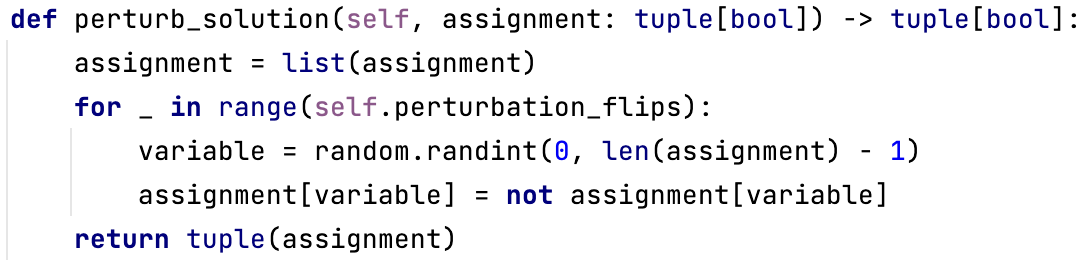
\includegraphics[width=7cm]{images/perturb}
        \caption{Perturbace ohodnocení proměnných}
        \label{fig:perturb}
    \end{figure}

    Algoritmus simulovaného ochlazování postupně odhlazuje aktuální teplotu.
    Na konci každé iterace je v hlavním cyklu volána metoda zobrazená na obrázku~\ref{fig:cool}.
    Chladící faktor je parametr heuristiky v rozsahu od 0 do 1, který je v následujících sekcích práce experimentálně nastaven
    na ideální hodnotu.

    \begin{figure}
        \centering
        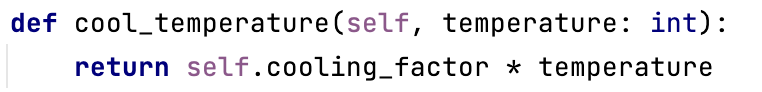
\includegraphics[width=7cm]{images/cool}
        \caption{Metoda pro chlazení teploty}
        \label{fig:cool}
    \end{figure}

    Při implementaci a testování heuristiky byly použity tyto testovací sady

    \begin{itemize}
        \item wuf20-71
        \item wuf20-71R
        \item wuf20-91
        \item wuf20-91R
        \item wuf50-200
        \item wuf50-219
        \item wuf50-218R
        \item wuf75-325
        \item wuf100-430
    \end{itemize}

    Parametry heuristy jsou následující

    \begin{itemize}
        \item \emph{initial\_temperature} - počáteční teplota
        \item \emph{final\_temperature} - konečná teplota
        \item \emph{num\_iterations\_per\_temperature} - počet iterací vnitřního cyklu ochlazování
        \item \emph{perturbation\_flips} - počet náhodně vybraných bitů pro flipnutí při prohledávání stavového prostoru
        \item \emph{cooling\_factor} - desetinné číslo (0, 1) reprezentující lineární funkci pro chlazení
        \item \emph{penalty} - celočíselná (záporná) hodnota penalizující nesplněnou klauzi (\emph{None} pro aktivaci adaptivní penalizace)
    \end{itemize}

%------------------------------------------------

    \section{White box testování}

    Jeden z prvních testů celého program odhalil závažnou chybu v programu.
    Chyba byla odhalena až po detailním výpisu grafu aktuálně nejlepších řešení heruistky.
    Teorie simulovaného ochlazování říka, že se snižující teplotou by se mělo řešení ustálit a zlepšovat.
    To na grafu zobrazeném na obrázku~\ref{fig:no-convergence} ale vůbec není patrné.

    Daný problém spočíval ve výpočtu a použití hodnoty delta (na obrázku~\ref{fig:main-loop}).
    Parametr delta se vypočítává odečtením hodnoty účelové funkce perturbovaného ohodnocení a hodnoty účelové funkce
    aktuálního ohodnocení.
    Následně je tato hodnota delta porovnána, zdali je větší než 0, což znamená zlepšení, v tom případě pertubované řešení
    nahrazuje aktuální ohodnocení a cyklus pokračuje dále.

    Problém nastával ale v~tom, že na parametru delta je také závislý výpočet pravděpodobnosti přijetí horšího řešení.
    V tomto případě je nutné počítat s~hodnotou delta v~absolutní hodnotě.
    Protože pro nízké teploty je tato delta velmi malá a zapříčinilo to přijetí mnoha zhoršujících řešení.
    Obrázek~\ref{fig:convergence} zobrazuje graf vývoje aktuálně nejlepšího řešení problému.
    Na tomto grafu je již vidět trend ochlazování a konvergence k optimálnímu řešení.

    \begin{figure}
        \centering
        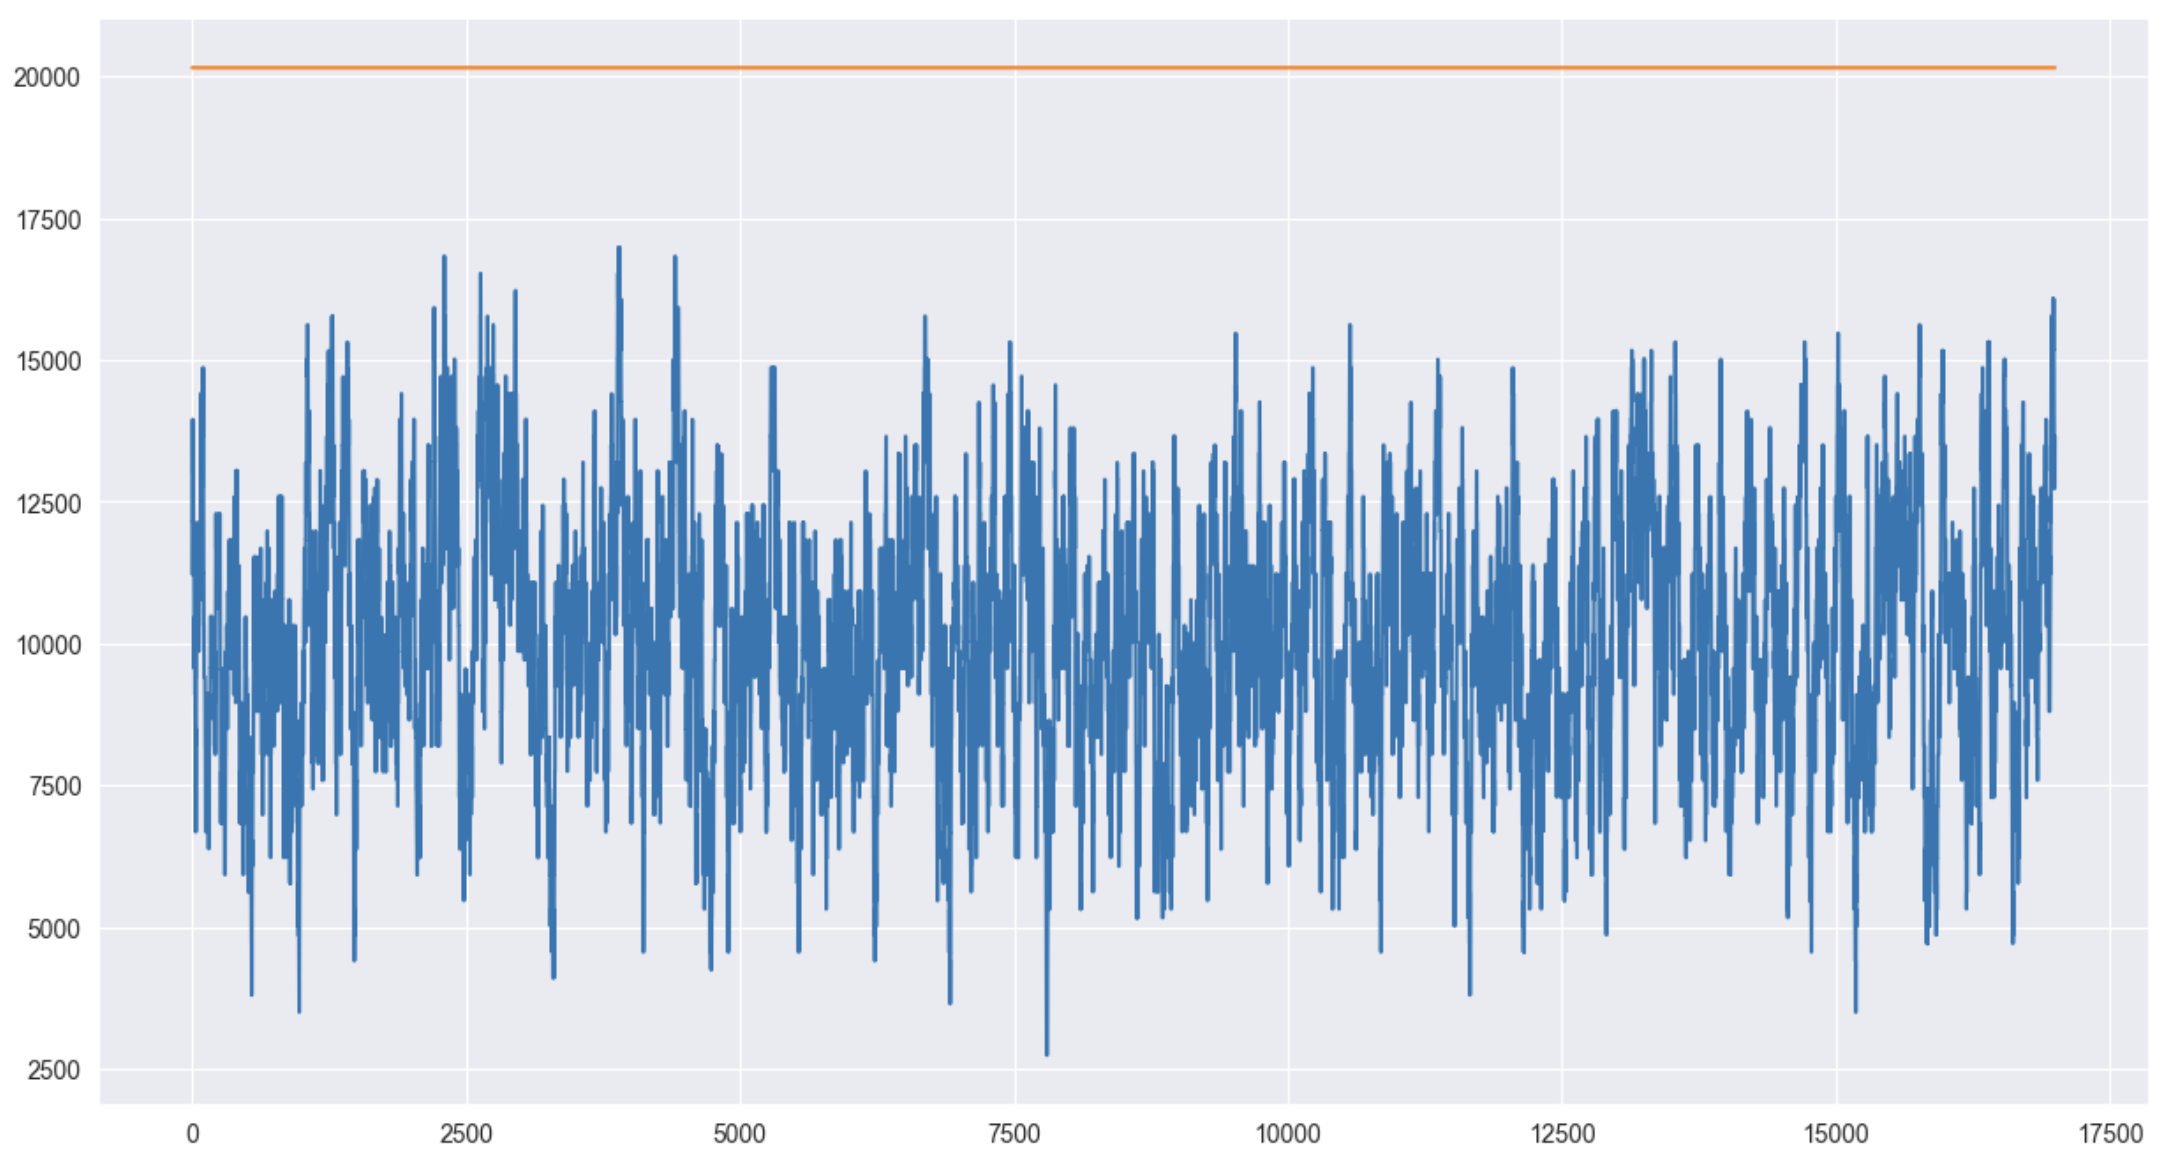
\includegraphics[width=7cm]{images/no-convergence}
        \caption{Simulované ochlazování bez konvergence}
        \label{fig:no-convergence}
    \end{figure}

    \begin{figure}
        \centering
        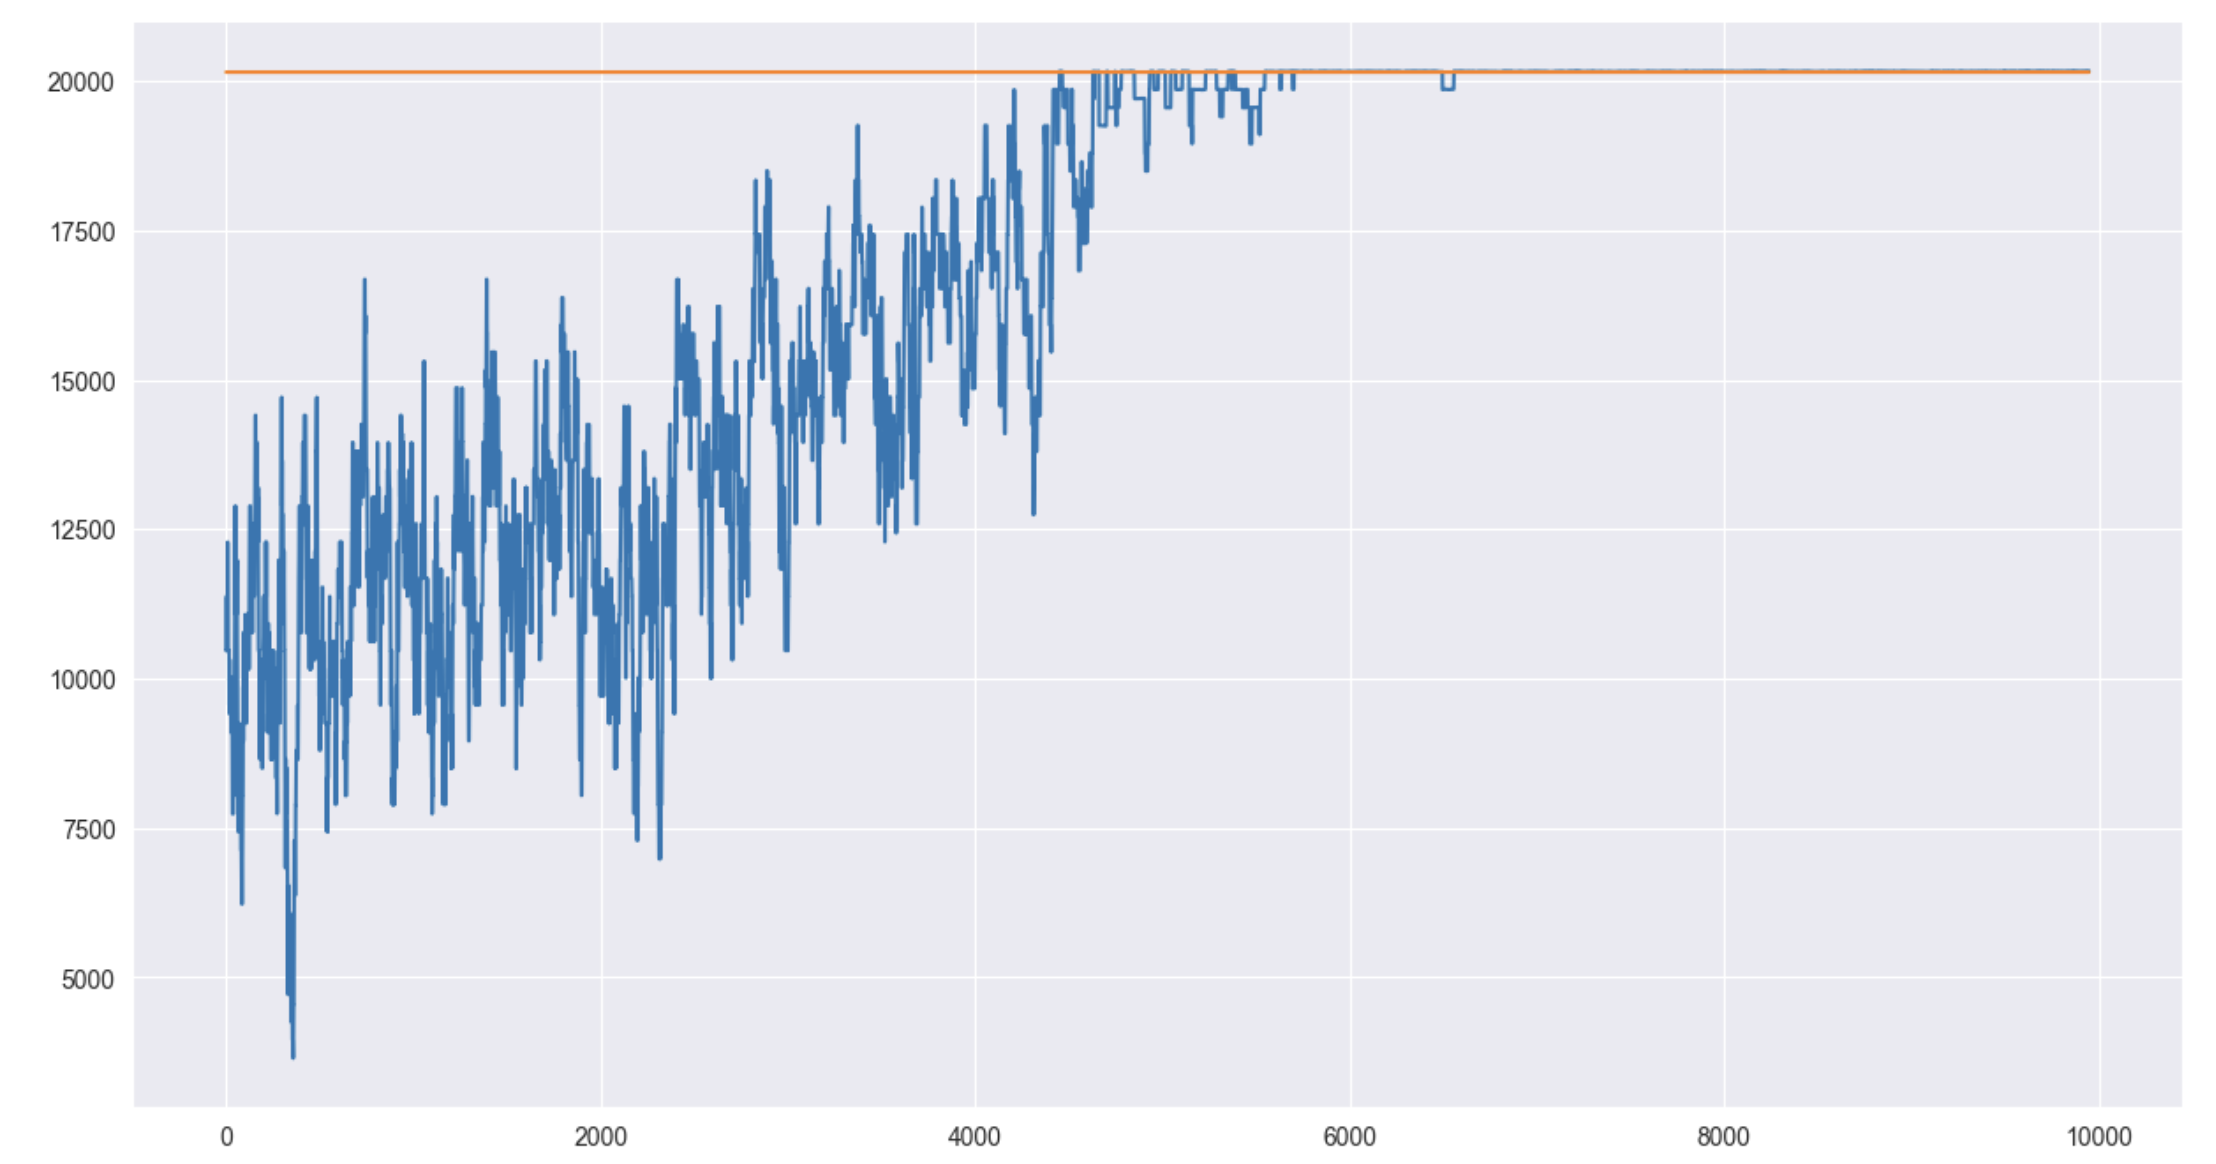
\includegraphics[width=7cm]{images/convergence}
        \caption{Simulované ochlazování s konvergencí}
        \label{fig:convergence}
    \end{figure}

    Následně byly testovány jednotlivé prametry heuristiky a závislost jejich nastavení na úspěšnosti nalezení optimálního řešení.
    Na náasledujících grafech je zobrazane úspěšnost nalezení optimálního řešení.
    Heuristika nalézá také neoptimální řešení, která jsou blízko optimálnímu, tato chyba zde však porovnána nebyla.

    Základním testem bylo nastavení počáteční teploty.
    Obrázky~\ref{fig:initial_temperature_71}~a~\ref{fig:initial_temperature_218R} zobrazují úspěšnosti nalezení optimálního řešení
    na instancích wuf20-71R a wuf50-218R s různými hodnotami počáteční teploty.
    Testované hodnoty byly z množiny

    \begin{itemize}
        \item 500
        \item 1000
        \item 2000
        \item 3000
        \item 4000
        \item 5000
        \item 6000
    \end{itemize}

    V těchto testech se hodnota 5000 jakožto počáteční teplota ukázala být nejvhodnější s~přihlédnutím na úspěšnost
    v~složitejších instancích a délce výpočetního času.

    \begin{figure}
        \centering
        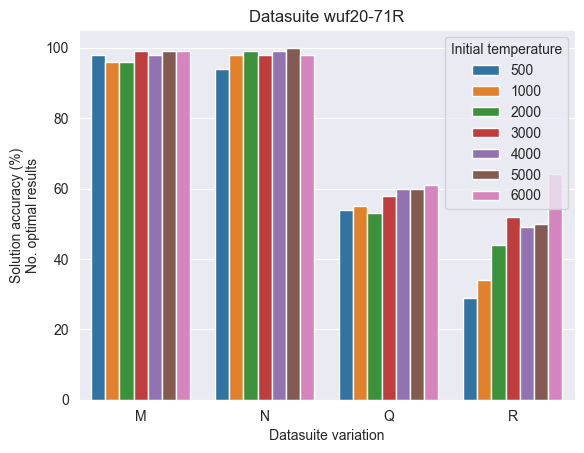
\includegraphics[width=7cm]{images/testing/initial_temperature/static_penalty_m5000/wuf20-71R}
        \caption{Experiment nastavení počáteční teploty 20-71R}
        \label{fig:initial_temperature_71}
    \end{figure}

    \begin{figure}
        \centering
        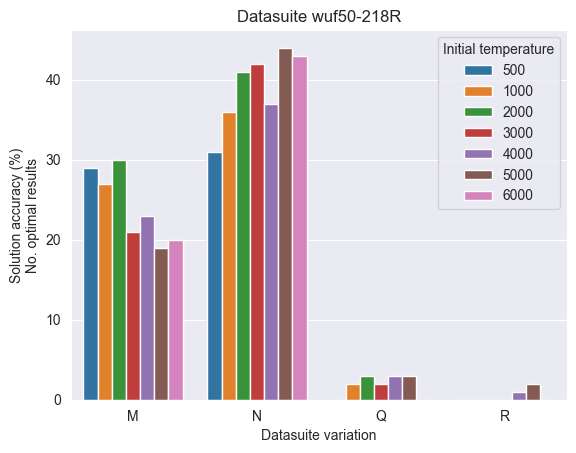
\includegraphics[width=7cm]{images/testing/initial_temperature/static_penalty_m5000/wuf50-218R}
        \caption{Experiment nastavení počáteční teploty 50-218R}
        \label{fig:initial_temperature_218R}
    \end{figure}

    Dále byla testován parametr chladícího faktoru.
    Tento parametr ovlivňuje rychlost konvergence metody a zároveň společně s nastavením počáteční a koncové teploty
    určuje počet kroků hlavního cyklu.

    Nastavení tohoto parametru bylo testováno na hodnotách

    \begin{itemize}
        \item .75
        \item .8
        \item .85
        \item .9
        \item .95
        \item .975
        \item .99
    \end{itemize}

    Grafy na obrázcích~\ref{fig:cooling_factor_71}~a~\ref{fig:cooling_factor_218R} zobrazují úspěšnost nalezení
    optimálního řešení v závislosti na nastavení hodnoty chladícího faktoru.

    \begin{figure}
        \centering
        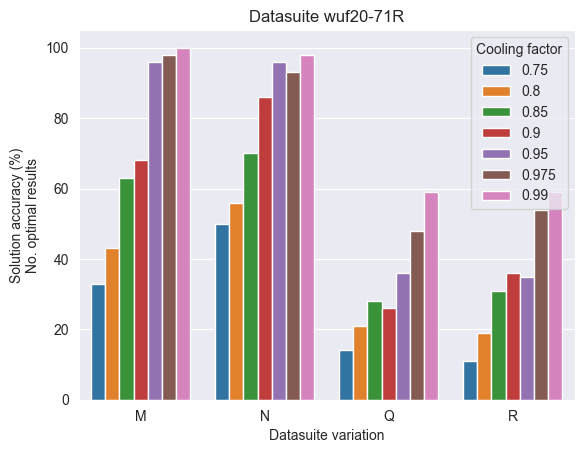
\includegraphics[width=7cm]{images/testing/cooling_factor/wuf20-71R}
        \caption{Experiment nastavení chladícího faktoru 20-71R}
        \label{fig:cooling_factor_71}
    \end{figure}

    \begin{figure}
        \centering
        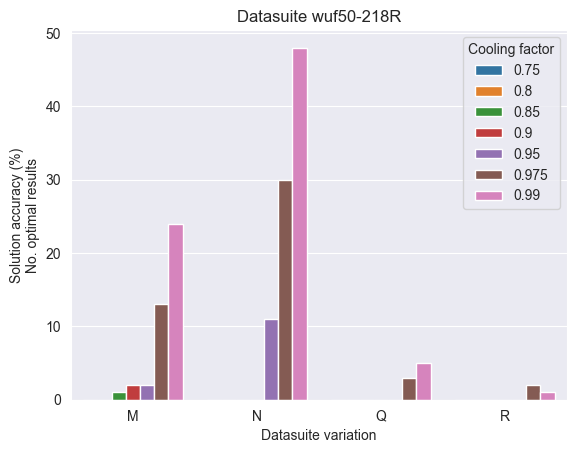
\includegraphics[width=7cm]{images/testing/cooling_factor/wuf50-218R}
        \caption{Experiment nastavení chladícího faktoru 50-218R}
        \label{fig:cooling_factor_218R}
    \end{figure}

%------------------------------------------------


    \section{Black box testování}

%------------------------------------------------


    \section{Závěr}

%----------------------------------------------------------------------------------------
%	REFERENCE LIST
%----------------------------------------------------------------------------------------

    \clearpage

    \bibliography{literature}
    \bibliographystyle{plain}

%\begin{thebibliography}{99} % Bibliography - this is intentionally simple in this template
%
%\bibitem[Figueredo and Wolf, 2009]{Figueredo:2009dg}
%Figueredo, A.~J. and Wolf, P. S.~A. (2009).
%\newblock Assortative pairing and life history strategy - a cross-cultural
%  study.
%\newblock {\em Human Nature}, 20:317--330.
%
%\end{thebibliography}

%----------------------------------------------------------------------------------------

\end{document}
